\documentclass[11pt]{article}

% ==== Paquetes ====
\usepackage[utf8]{inputenc}
\usepackage[spanish]{babel}
\usepackage[T1]{fontenc}
\usepackage{amsmath, amssymb, amsfonts, siunitx}
\usepackage{graphicx}
\usepackage{float}
\usepackage{xcolor}
\usepackage{hyperref}
\usepackage{caption}
\usepackage{subcaption}
\usepackage{geometry}
\usepackage{listings}
\usepackage{pdfpages}
\usepackage{tikz}

\definecolor{codegreen}{rgb}{0,0.6,0}
\definecolor{codegray}{rgb}{0.5,0.5,0.5}
\definecolor{codepurple}{rgb}{0.58,0,0.82}
\definecolor{backcolour}{rgb}{0.95,0.95,0.92}

\lstset{
  inputencoding=utf8,
  extendedchars=true,
  literate=
   {á}{{\'a}}1 {é}{{\'e}}1 {í}{{\'i}}1 {ó}{{\'o}}1 {ú}{{\'u}}1
   {Á}{{\'A}}1 {É}{{\'E}}1 {Í}{{\'I}}1 {Ó}{{\'O}}1 {Ú}{{\'U}}1
   {ñ}{{\~n}}1 {Ñ}{{\~N}}1
   {¿}{{?`} }1 {¡}{{!`} }1
}

\lstdefinestyle{mystyle}{
    backgroundcolor=\color{backcolour},   
    commentstyle=\color{codegreen},
    keywordstyle=\color{magenta},
    numberstyle=\tiny\color{codegray},
    stringstyle=\color{codepurple},
    basicstyle=\ttfamily\footnotesize,
    breakatwhitespace=false,         
    breaklines=true,                 
    captionpos=b,                    
    keepspaces=true,                 
    numbers=left,                    
    numbersep=5pt,                  
    showspaces=false,                
    showstringspaces=false,
    showtabs=false,                  
    tabsize=2,
    upquote=true,
    inputencoding=utf8,
}

\lstset{style=mystyle}

\geometry{margin=2.5cm}

% ==== Datos de la tarea ====
\title{IEE3584 - Procesamiento Avanzado de Señales \\
Tarea 4}
\author{Nicolás Seguel}
\date{Septiembre 2025}

\begin{document}

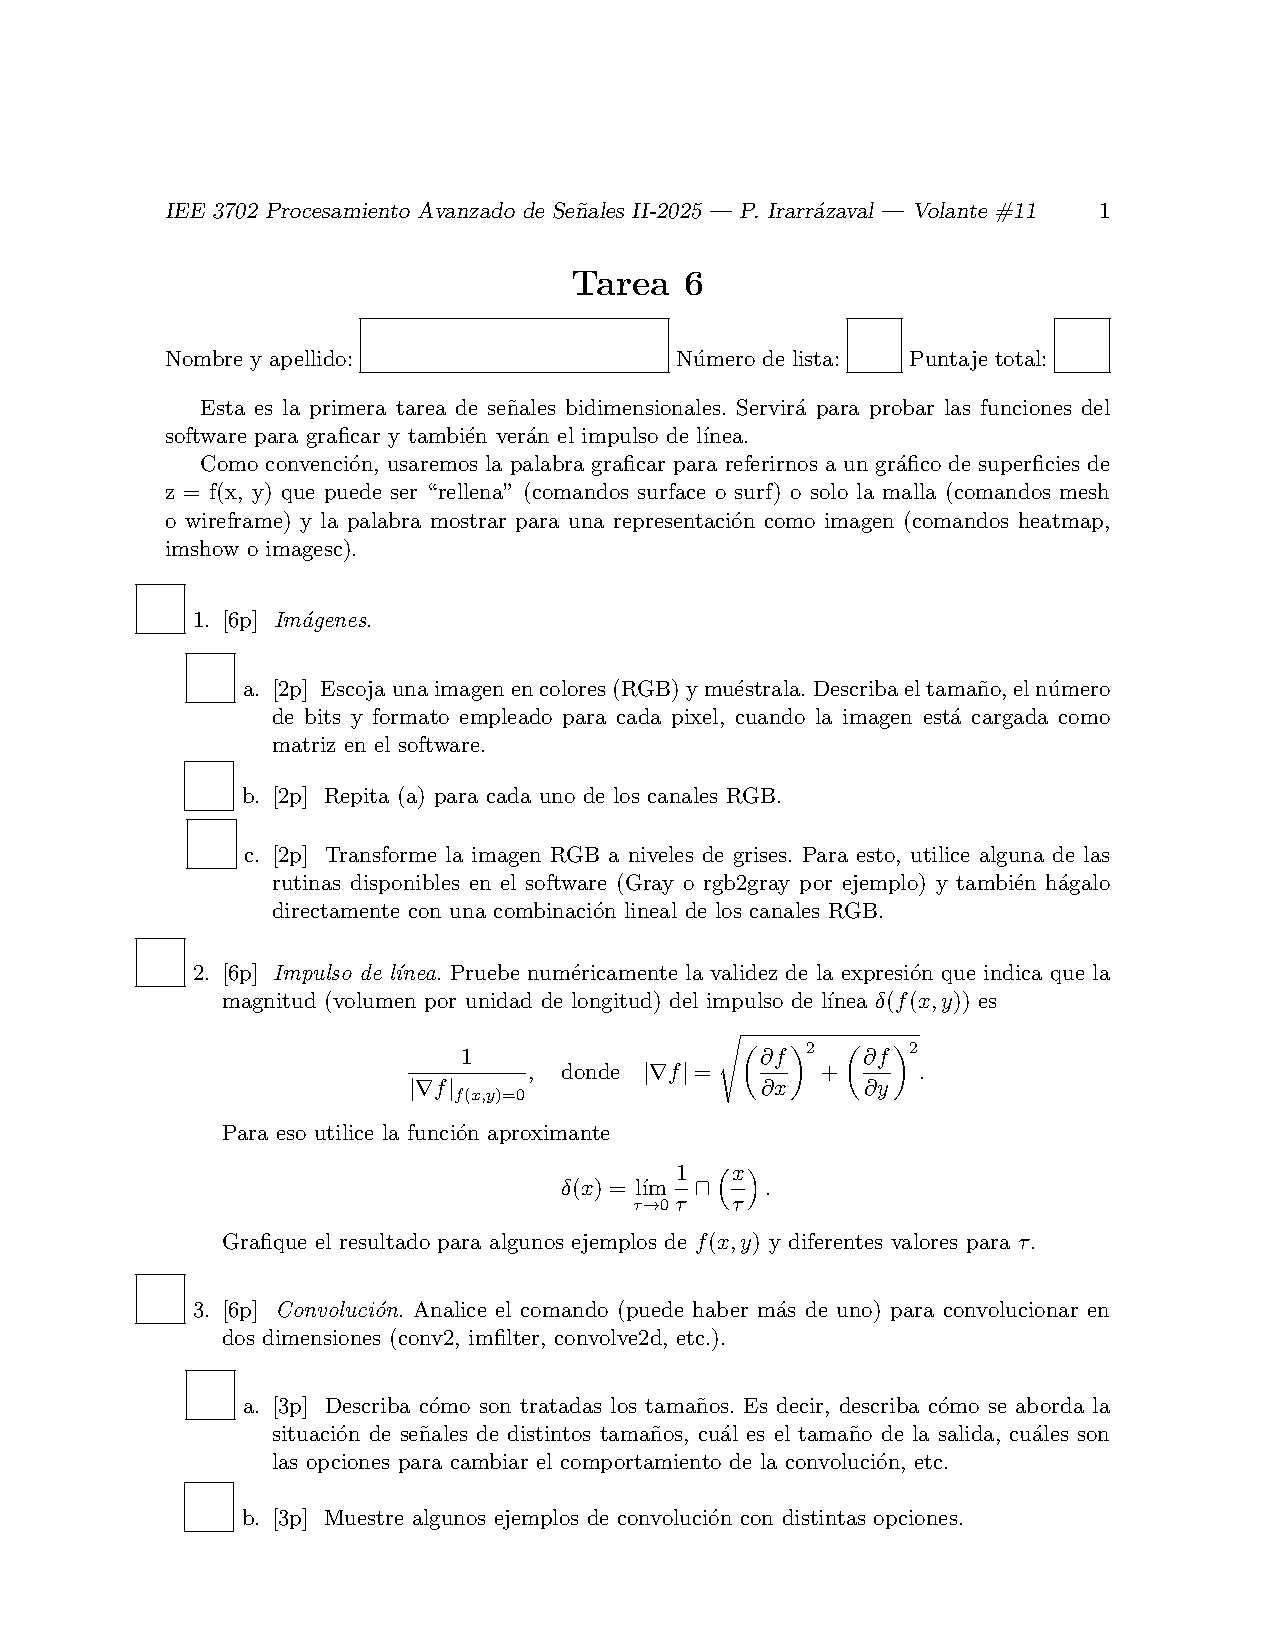
\includepdf[pages=-]{11.tarea06.pdf}
\maketitle

% ==== Problema 1 ====
\section*{1. \textit{Imágenes}}

\subsection*{a.}

Se cargó una imagen de 1200 por 1599 pixeles. El formato de cada pixel es \texttt{float64} por lo que tienen 64 bits de información.

\begin{figure}[H]
    \centering
    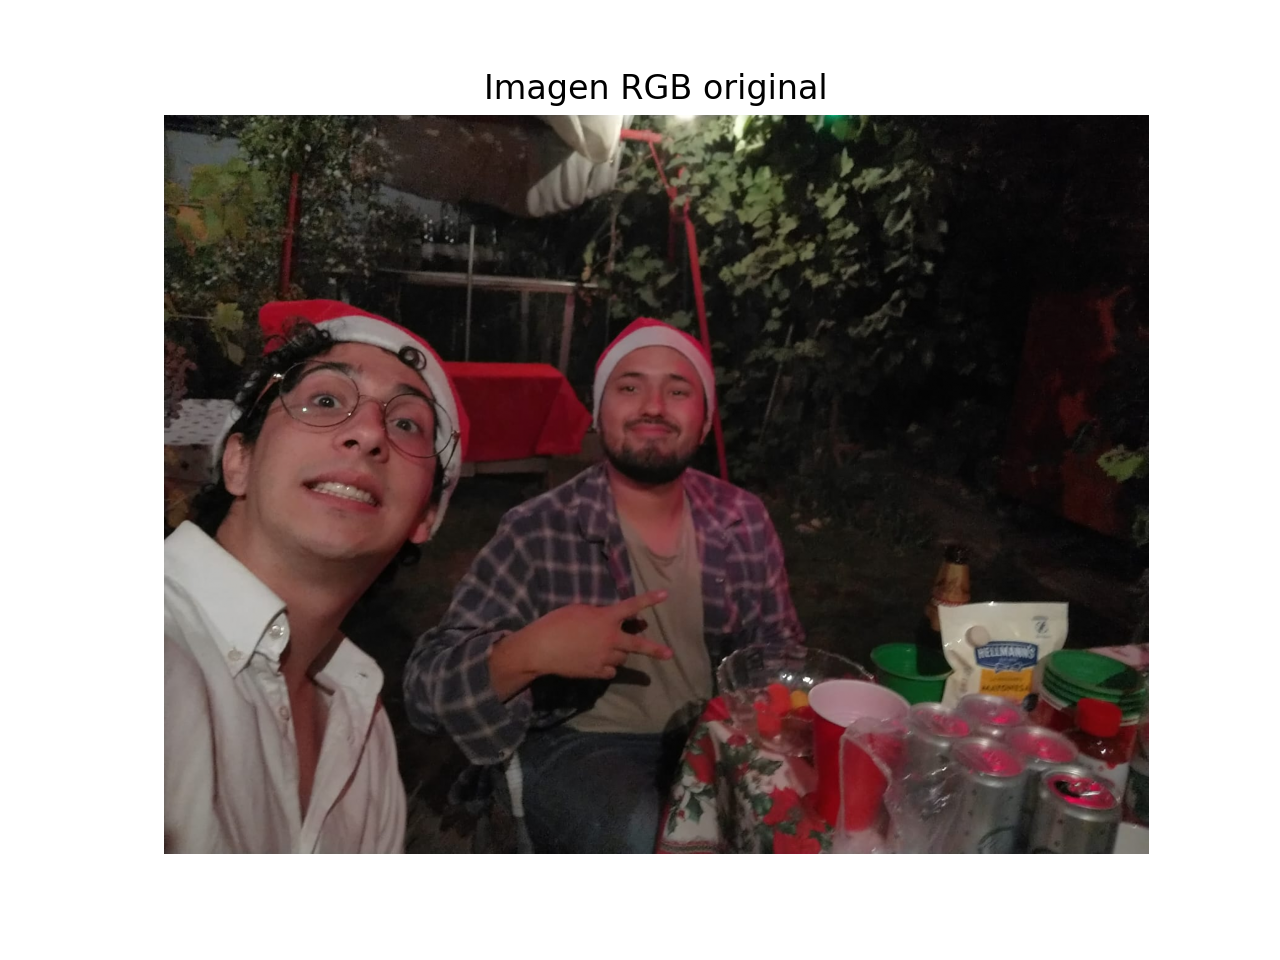
\includegraphics[width=0.5\textwidth]{figs/p1a_imagen_rgb.png}
    \caption{Imagen RGB original.}
\end{figure}

\subsection*{b.}
\begin{figure}[H]
    \centering
    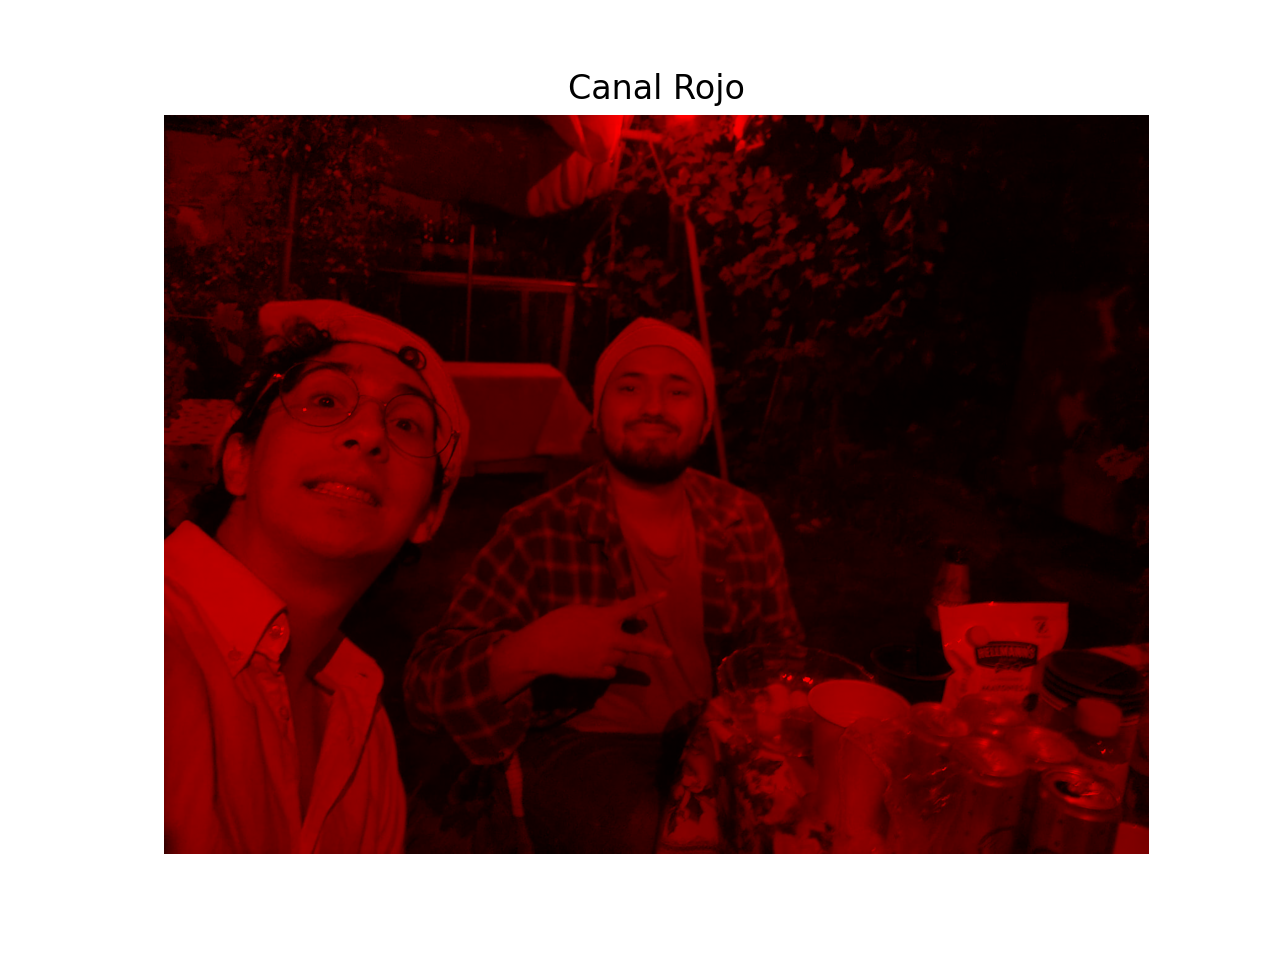
\includegraphics[width=0.32\textwidth]{figs/p1b_canal_rojo.png}
    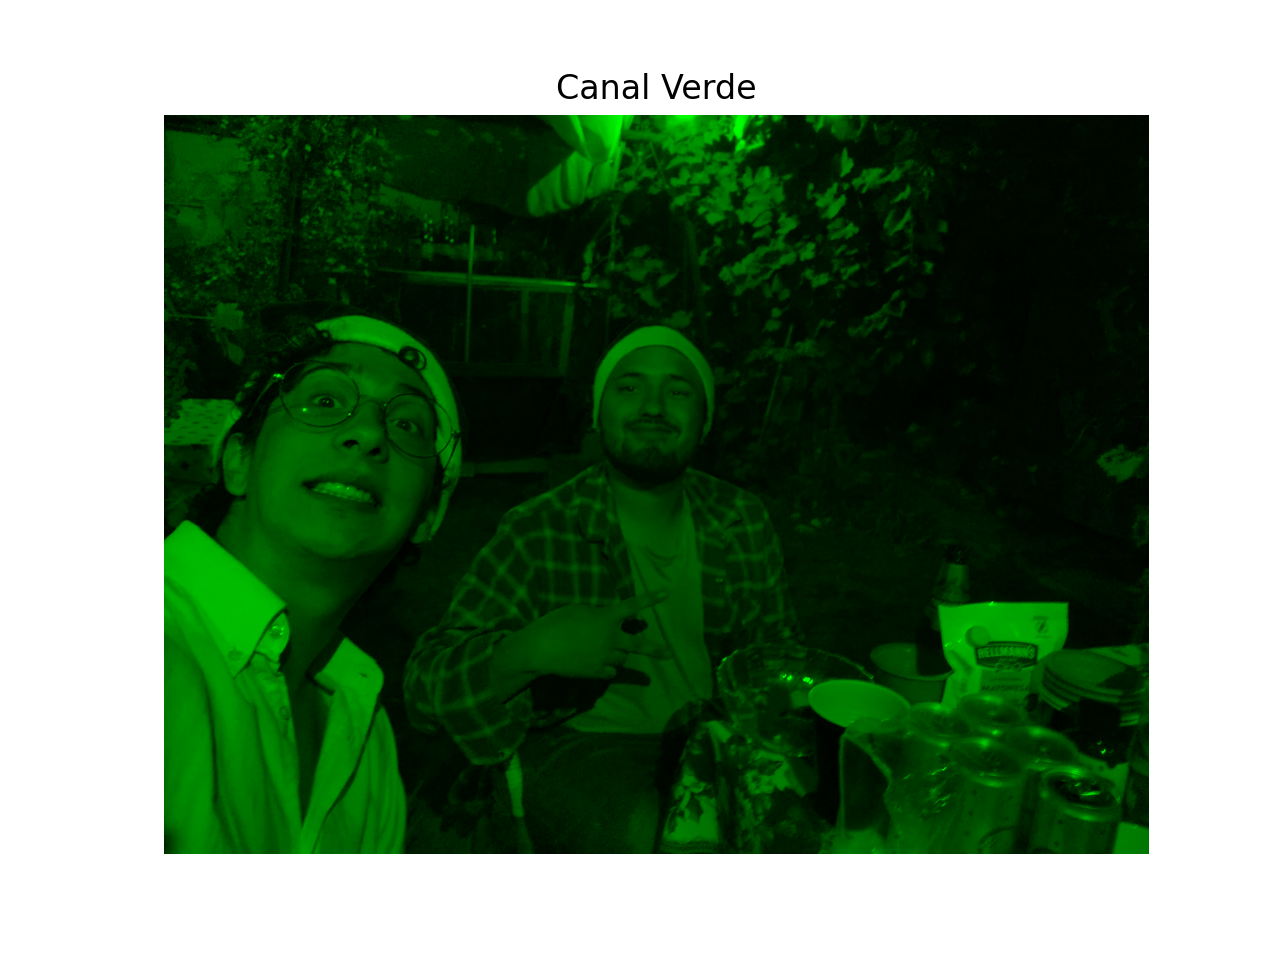
\includegraphics[width=0.32\textwidth]{figs/p1b_canal_verde.png}
    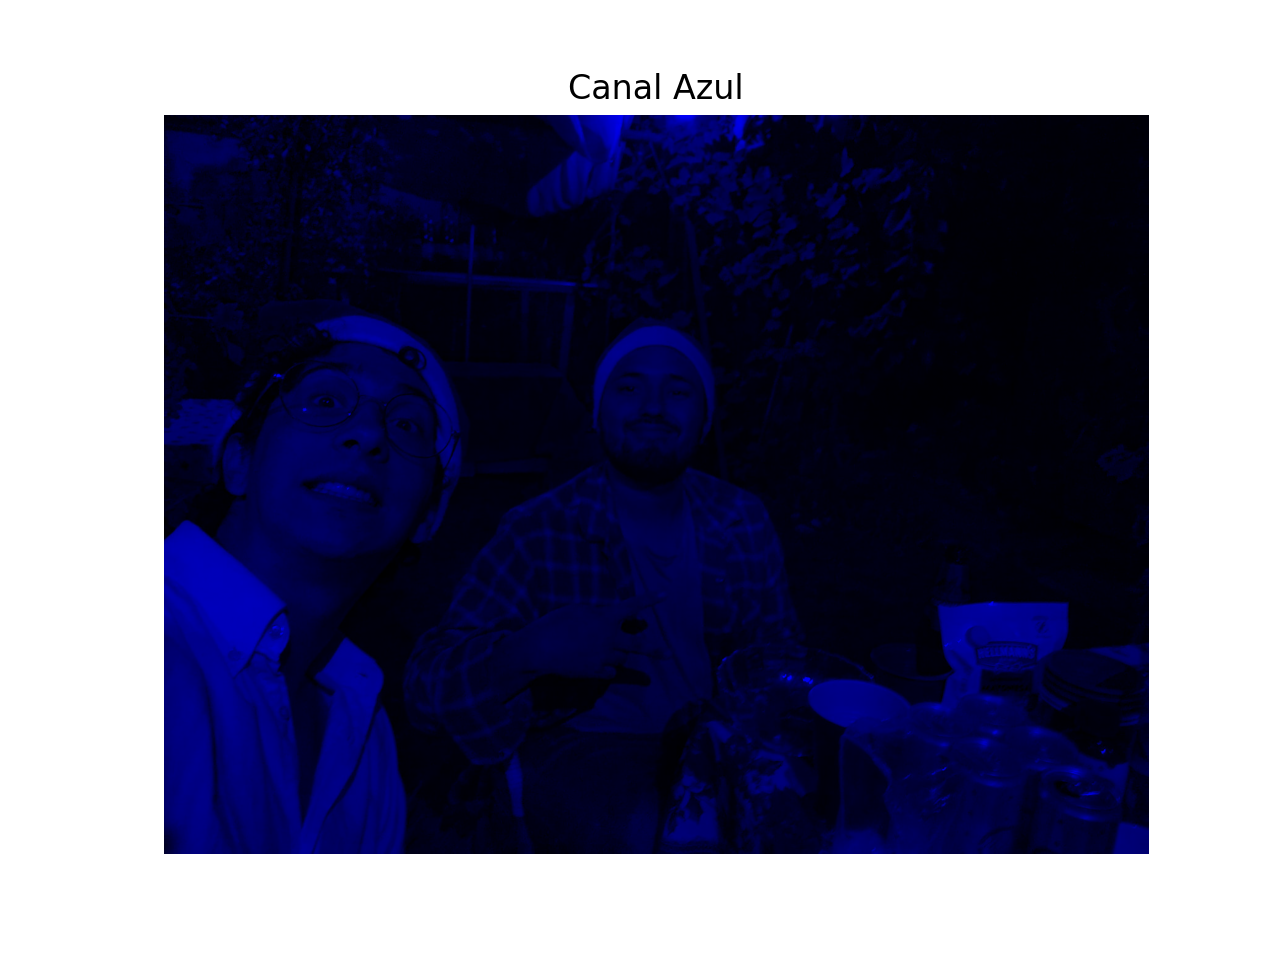
\includegraphics[width=0.32\textwidth]{figs/p1b_canal_azul.png}
    \caption{Canales individuales R, G, B.}
\end{figure}

\subsection*{c.}
\begin{figure}[H]
    \centering
    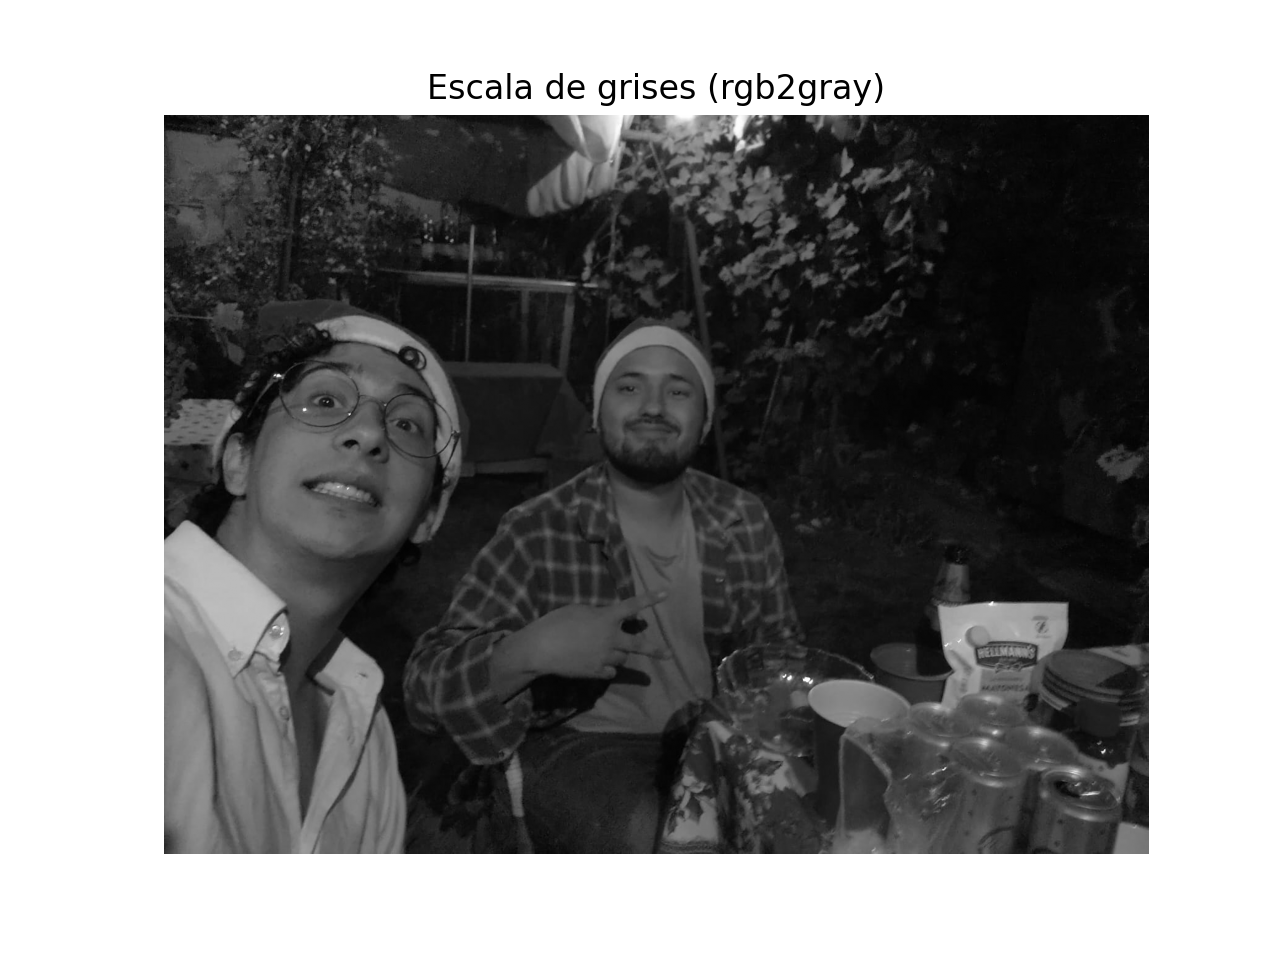
\includegraphics[width=0.45\textwidth]{figs/p1c_grises_funcion.png}
    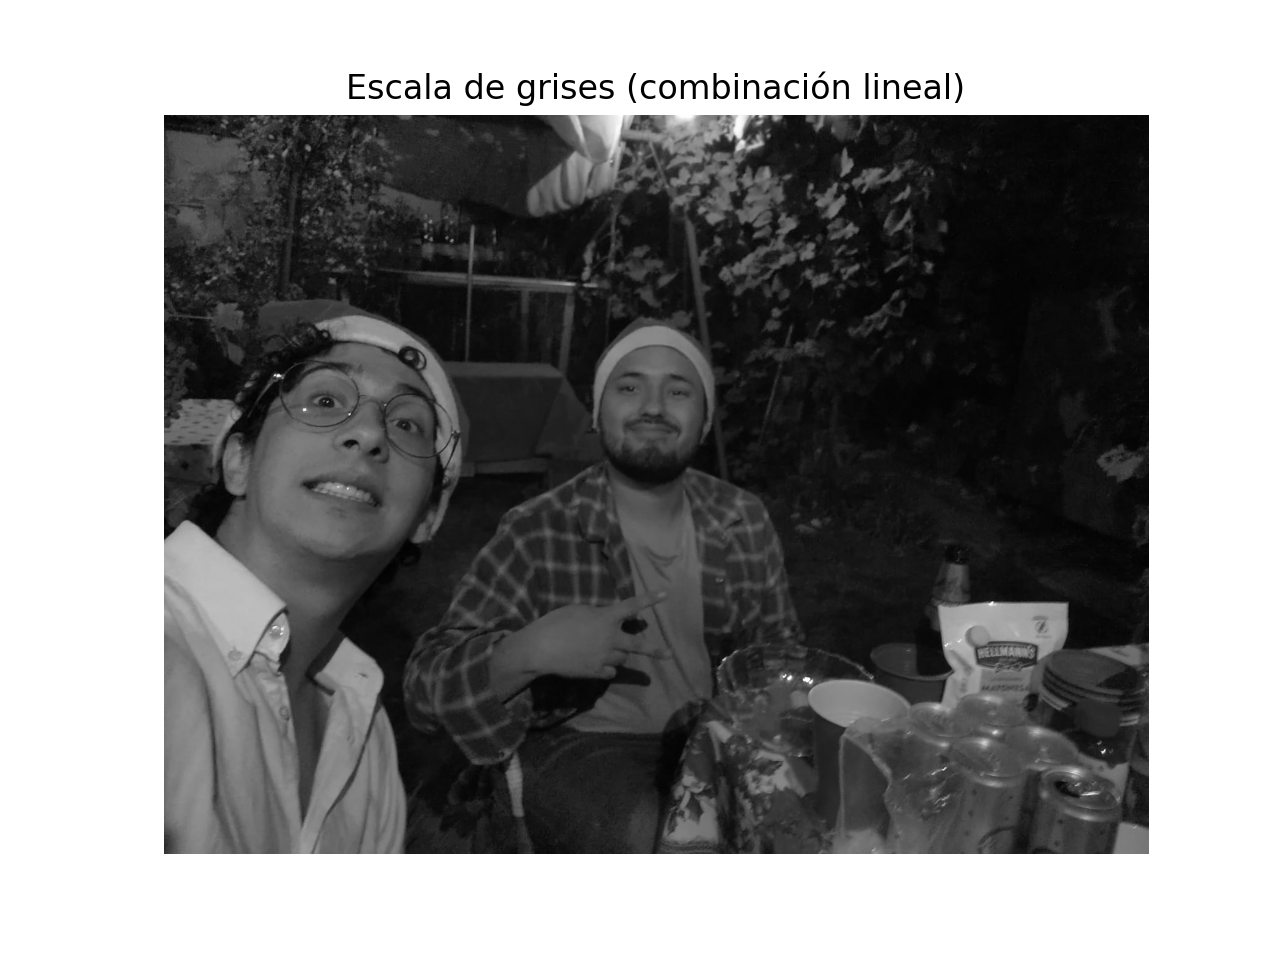
\includegraphics[width=0.45\textwidth]{figs/p1c_grises_manual.png}
    \caption{Conversión a escala de grises por función y por combinación lineal.}
\end{figure}

\lstinputlisting[
    style=mystyle,
    language=Python,
    caption={Archivo \texttt{pregunta1.py}}
]{pregunta1.py}


% ==== Problema 2 ====
\section*{2. \textit{Impulso en línea}}

\begin{figure}[H]
    \centering
    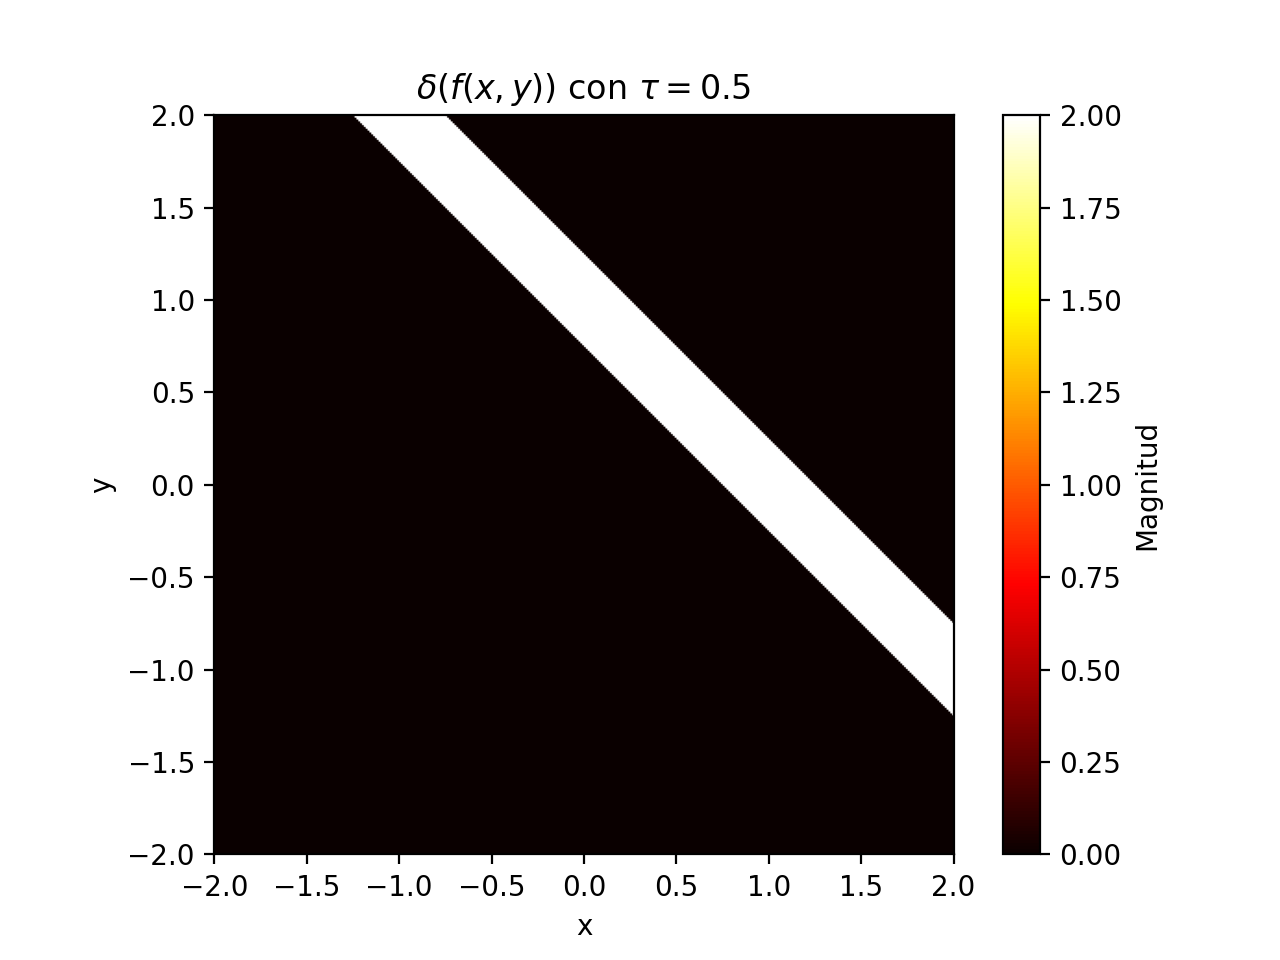
\includegraphics[width=0.32\textwidth]{figs/p2_impulso_tau0.5.png}
    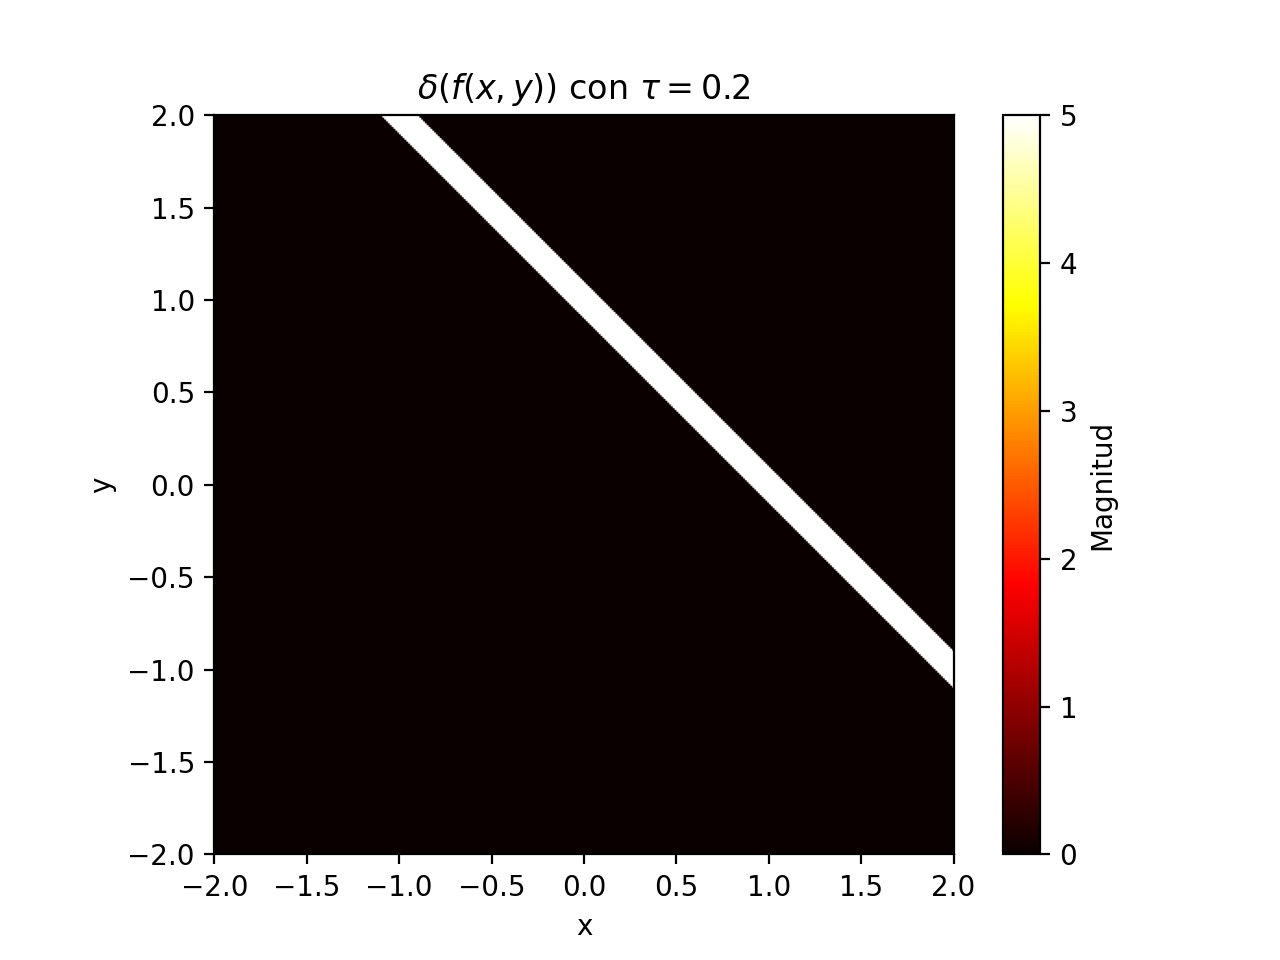
\includegraphics[width=0.32\textwidth]{figs/p2_impulso_tau0.2.png}
    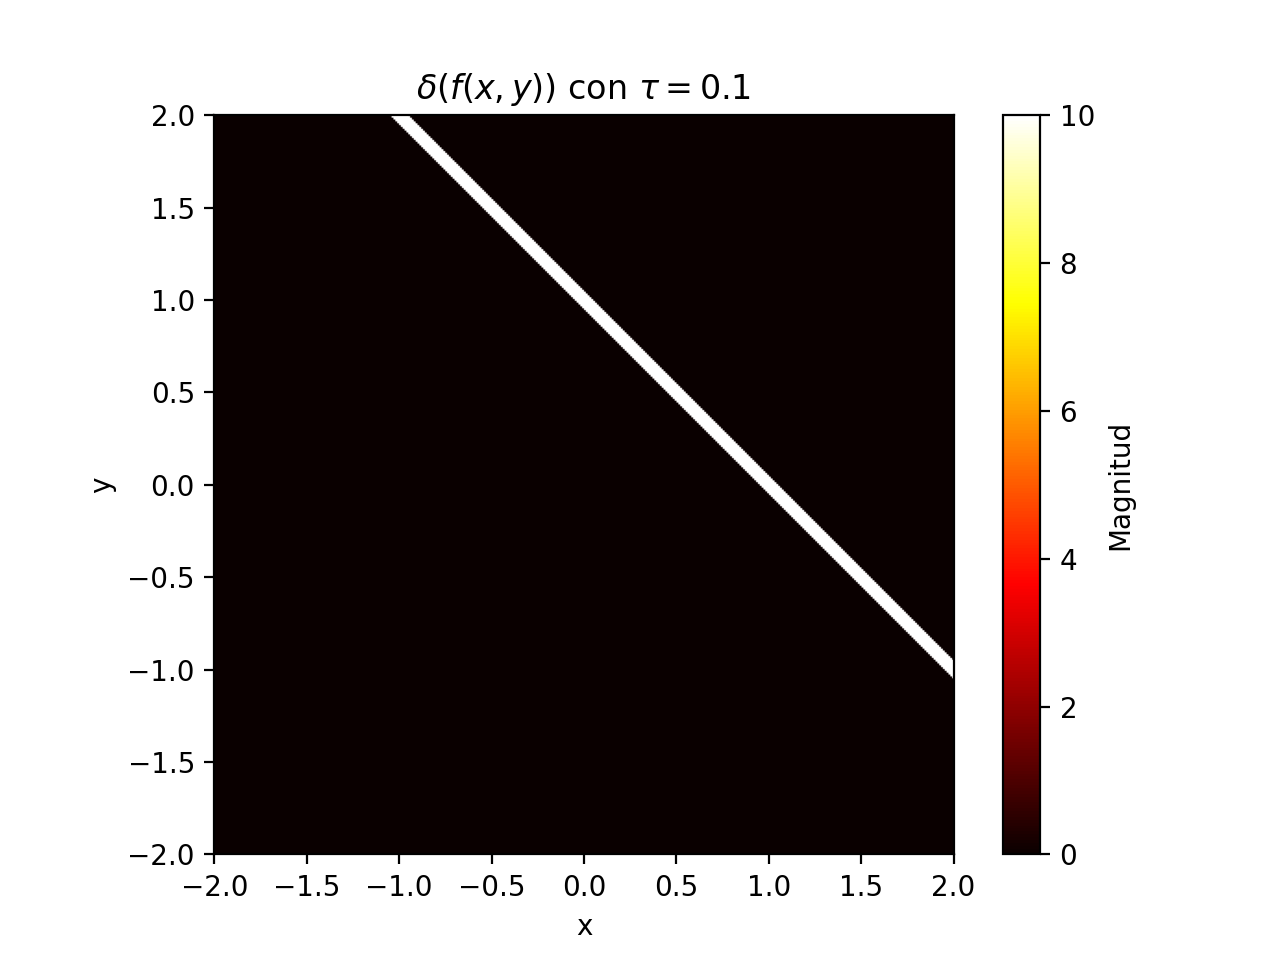
\includegraphics[width=0.32\textwidth]{figs/p2_impulso_tau0.1.png}
    \caption{Aproximaciones del impulso de línea para distintos valores de $\tau$.}
\end{figure}

\lstinputlisting[
    style=mystyle,
    language=Python,
    caption={Archivo \texttt{pregunta2.py}}
]{pregunta2.py}

% ==== Problema 3 ====
\section*{3. \textit{Convolución}}

\subsection*{a.}

\subsection*{b.}

\begin{figure}[H]
    \centering
    
\includegraphics[width=0.25\textwidth]{figs/p3_imagen_original.png}
    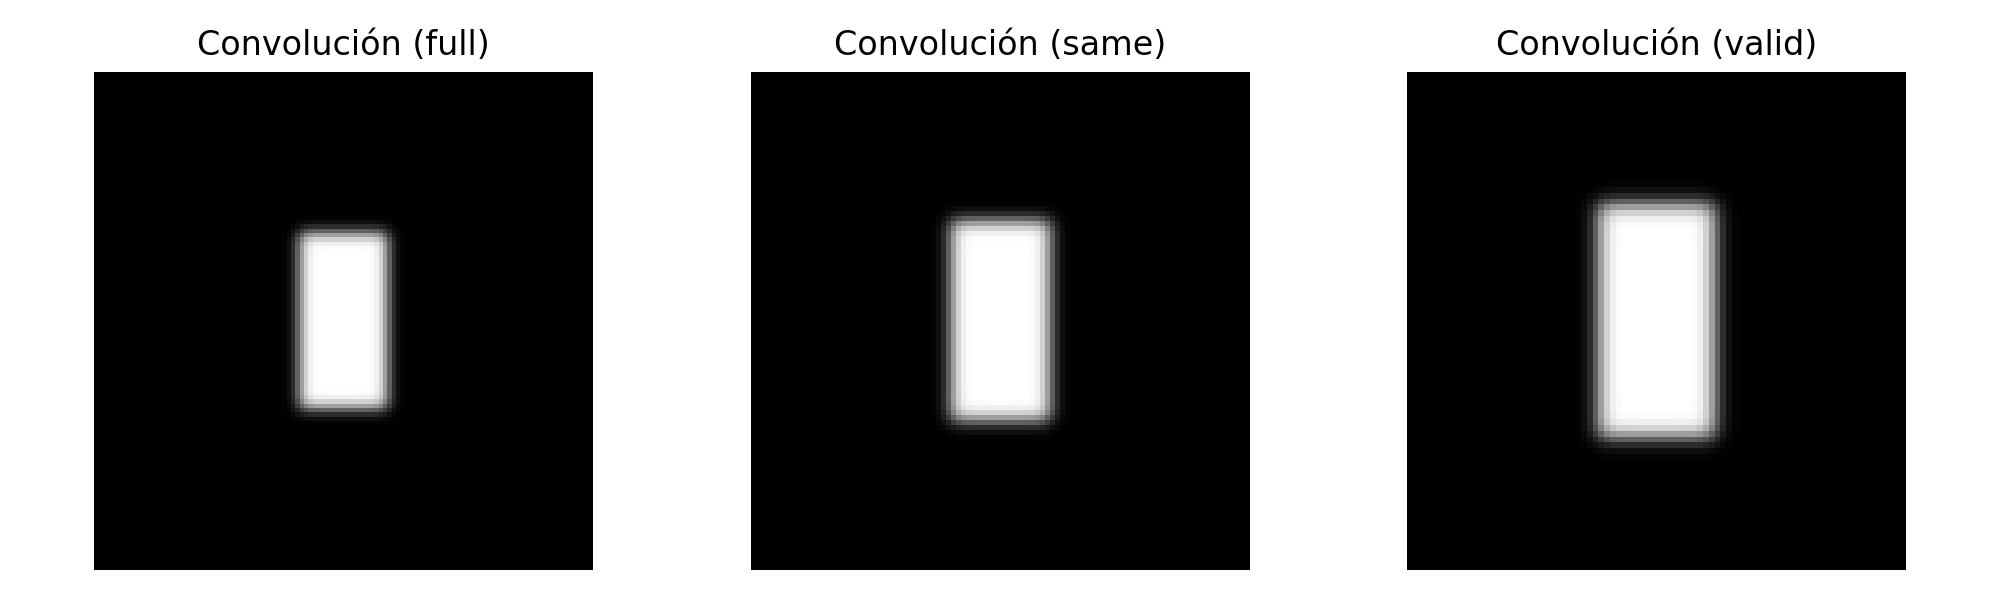
\includegraphics[width=0.7\textwidth]{figs/p3_convoluciones.png}
    \caption{Convolución 2D con distintas opciones de tamaño.}
\end{figure}

\lstinputlisting[
    style=mystyle,
    language=Python,
    caption={Archivo \texttt{pregunta3.py}}
]{pregunta3.py}

\end{document}